\chapter{Mathematical Background\label{ch:math}}

	This chapter aims to give a thorough introduction to the mathematical ideas necessary to cast the geometric Langlands program and gauge theory in a coherent framework. 
	
	
	
	\section{Finite Dimensional Linear Algebra} % (fold)
	\label{sec:finite_dimensional_linear_algebra}
	
	We begin with a study of elementary representation theory, first through the familiar lens of eigenvalues in linear algebra, and then by studying the representations of a group. We assume the reader is familiar with these fields, and include them both as motivation and for completeness. The representation theory of finite (or more generally locally-compact) abelian groups is a straightforward generalization of the ideas of the Fourier transform. 
	
	More broadly, for someone with a background in engineering, representation theory itself can be viewed as one tremendous generalization of Fourier analysis. 
	Through this naive lens, many of the dualities explored in this paper are great generalizations of the duality between the domains of time and frequency, position and momentum, shape and spectrum, etc. 
	
	
		
		The role of eigenvalues is central across pure and applied mathematics, engineering, market-making, physics, network theory, neuroscience, etc. In many scenarios, one has a system with multiple components that interact/transfer energy between one another. The state of the system of $n$ components is specified by an $n$-component \textbf{vector} $\mathbf v$, often of real or complex numbers, that we say lies in the \textbf{vector space} $V = \mathbf k^n$ of $n$-tuples of numbers valued in the \textbf{ground field} $\mathbf k$. 
		% More generally, we say that
% 		\begin{defn}[Vector Space]
% 			A vector space over a field $\mathbf k$ is a set $V$ together with the commutative operation of vector addition and scalar multiplication so that $a \mathbf v + b \mathbf w \in V$ and $a \mathbf v \in V$ for all vectors $\mathbf v, \mathbf w \in V$.
%
% 			A subset of a vector space closed under these operations is called a \textbf{subspace}.
% 		\end{defn}
		
		A natural morphism\footnote{See appendix on category theory.} of vector spaces is a \textbf{linear transformation}, taking us from one vector space $V$ to another $W$, denoted $T: V \to W$ satisfying
		$$\forall \mathbf v_1, \mathbf v_2 \in V, a, b \in \mathbf k, \qquad  T(a \mathbf v_1 + c \mathbf v_2) = a T(\mathbf v_1) + b T(\mathbf v_2).$$
		If a basis is chosen for space, these transformations can be written as matrices. Of particular interest are the linear transformations taking us from $V$ to $V$, also known as the \textbf{endomorphisms} of $V$. 
		
		In the following, let $V$ be finite-dimensional.
		The simplest endomorphisms are simply the actions of scalar multiplication $\mathbf v \to \lambda \mathbf v, \lambda \in \mathbf k$. Here, the study of linear algebra trivializes to become the study of nothing more than multiplication. A linear transformation that acts as scaling on every vector on the space is called \textbf{simple}.
		
		The next simplest class of endomorphisms are those that act as (possibly distinct) scalars on the elements of some basis $\mathbf v_i$. Namely, in the basis $\{ \mathbf v_i \}$, such an operator $T$ can be written as:
		\begin{equation}T \to
			\begin{pmatrix}
				\lambda_1 & 0 & \dots & 0\\
				0 & \lambda_2 & \dots & 0\\
				\vdots & \vdots & \ddots & \vdots\\
				0 & 0 & \dots & \lambda_n
			\end{pmatrix}
		\end{equation}
		Such matrices are commonly called \textbf{diagonalizable}, but to emphasize a similarity with later topics, we remark that another term for them is \textbf{semisimple}. 
		\begin{defn}[Spectrum of a Semisimple Operator]
		For a semisimple operator $T$ the set of eigenvalues, \emph{counted with multiplicity}, is called its \textbf{spectrum}\footnote{The origin of this term comes from early quantum mechanics, in which the eigenvalues of the matrix mechanics of Heisenberg produced accurate predictions of the electromagnetic spectra of atoms.} and denoted $\spec{T}$.
		\end{defn}
		Along with this definition, we recall what it means to form a \textbf{direct sum}. 
		\begin{defn}[Direct Sum of Vector Spaces]
			Given two vector spaces $V_1, V_2$, their direct sum $V_1 \oplus V_2$ is a vector space $V$ so that every vector $\mathbf v \in V$ can be written \emph{uniquely} as $\mathbf v = \mathbf v_1 + \mathbf v_2$ for $\mathbf v_1 \in V_1, \mathbf v_2 \in V_2$.
		\end{defn}
		The reason we use the term `semisimple' instead of the easier `diagonalizable' is because the vector space $V$ decomposes into a direct sum of \textbf{eigenspaces}
		\begin{equation}
			V = \bigoplus_{\lambda \in \spec{T}} V_{\lambda}
		\end{equation}
		 on which $T$ as a simple transformation: multiplication by $\lambda_i$. In general, the spectrum of a transformation can be extracted by finding when $T - \lambda I = 0$ on some subspace. Having a nonzero kernel will necessitate that $\det (T - \lambda I) = 0$. When this is viewed as a polynomial in $\lambda$ it yields the \textbf{characteristic polynomial} of $T$. The characteristic polynomial is independent of the basis that $T$'s matrix form is represented in.
		
		Not all linear transformations are diagonalizable. A simple example of a transformation $T$ that is not diagonalizable is one that has a matrix
		$$\begin{pmatrix}
			0 & 1\\
			0 & 0
		\end{pmatrix}$$ 
		The solutions of the characteristic polynomial are $\lambda^2 = 0$, namely we expect the two eigenvalues to both be zero. On the other hand, it is easy to see that \emph{only} the vector $(1, 0)$ is an eigenvector of this operator. 
		\begin{defn}[Nilpotent Operator]
			A \textbf{nilpotent} operator $T$ satisfies $T^k = 0$ for some $1 \leq k \leq \dim V$.
		\end{defn}
		Any nilpotent operator will have characteristic polynomial of the form $\lambda^n = 0$ where $n = \dim V$, but (unless it is the zero matrix) will not have $n$ independent eigenvectors. This prevents it from being semisimple in general.
		
		Notice that in the above example, $T$ acting on $(0, 1)$ produces $(1, 0)$, which when acted on by $T$ again will vanish. This is the general idea of nilpotent operators. Since their determinant is zero, they necessarily have a subspace $V_1$ on which $T|_{V_1} = 0$, and because $T^k = 0$ for some $1 \leq k \leq n$, any vector will eventually be sent to zero after repeated application of $T$, meaning any vector space will eventually be sent inside $T_{1}$. This gives us a stratification of $V$:
		
		\begin{equation}
			0  = V_0 \subset V_1 \subset V_2 \subset \dots \subset V_k = V, \qquad V_i := \ker T^i
		\end{equation}
		it is easy to see that inclusions must be strict, otherwise $T$ would stabilize a subspace, contradicting nilpotenency. Such a stratification is called a \textbf{flag} in $V$. 
		\begin{defn}[Flag]
			A flag in a vector space $V$ is an increasing sequence of subspaces $V_i$ of $V$ such that each space is a \emph{proper} subspace of the next. If each $V_i$ is codimension $1$ inside of $V_{i+1}$, then $k = n$ and this is called a \textbf{complete flag}.
		\end{defn}
		Subspaces are themselves special (almost trivial) cases of flags. In this light, flags can be seen as a generalization of the notion of subspaces, and play a significant role in representation theory, to be discussed later.
		
		
		 On finite-dimensional vector spaces, nilpotent operators play the roles of `raising' and `lowering' operators in quantum mechanics (see next chapter). A lowering matrix takes the form:
		 $$\small \begin{pmatrix}
		 	0 & 1 & 0 & \dots & 0\\
			0 & 0 & 1 & \dots & 0\\
			\vdots & \vdots & \ddots & \ddots & \vdots\\
			0 & 0 & 0 & \ddots & 1\\
			0 & 0 & 0 & \dots & 0
		 \end{pmatrix}$$
		
		\begin{theorem}[Classification of Nilpotent Operators]
			Given a nilpotent operator $T$, we can find a basis and decompose $V$ into a direct sum $V = \bigoplus_{i} V_i$ on which $T$ acts as a lowering operator.
		\end{theorem}
		
		
		From our knowledge of semisimple and nilpotent operators, we can state the following theorem:
		\begin{theorem}[Jordan Normal Form]
			Every linear operator on a finite dimensional vector space over $\mathbb C$ can be decomposed as a sum of a semisimple one and a nilpotent one. 
			
			Equivalently, every linear operator has an \textbf{eigenbasis} in which it can be written in \textbf{Jordan normal form}:
			\begin{equation}\small
				\begin{pmatrix}
					J_1 & 0 & \dots & 0 \\
					0 & J_2 & \dots & 0\\
					\vdots & \vdots & \ddots & \vdots\\
					0 & 0 & \dots & J_k \\
				\end{pmatrix}
			\end{equation}
			Where each $J_i$ is an $\ell_i \times \ell_i$ matrix called a \textbf{Jordan block} taking the form:
			\begin{equation}\small
				\begin{pmatrix}
					\lambda_i & 1 & 0 & \dots & 0 & 0 \\
					0 & \lambda_i & 1 & \dots & 0 &0 \\
					\vdots & \vdots & \vdots & \ddots & \vdots & \vdots\\
					0 & 0 & 0 & \dots & \lambda_i & 1 \\
					0 & 0 & 0 &\dots & 0 & \lambda _i
				\end{pmatrix}.
			\end{equation}
			We say $\ell_i$ is the length of the $i$th Jordan block.
			
			It is clear that if each Jordan block has length 1, the matrix is diagonalizable, i.e. semisimple.
		\end{theorem}

		Overall, linear operators on a vector space over an algebraically closed field fall into the hierarchy diagrammed in Figure~\ref{fig:JNF}.
		\begin{center}
		\begin{figure}[h]
			\[
			\begin{tikzcd}
			   & & 0\arrow[ld] \arrow[rd] & &\\
			  \text{Eigenspace} & \arrow[l,dashed] \parbox{3em}{Simple\\($\lambda \cdot 1$)} \arrow[dd,"\bigoplus"]\arrow[rd] & & \text{Raising} \arrow[dd,"\bigoplus"]\arrow[ld] \arrow[r,dashed] & \text{Complete Flag} \\
			  & & \text{\textit{Jordan Blocks}} \arrow[dd,"\bigoplus"] & &\\
			  \parbox{5em}{Eigenspace\\ Decomposition}&\parbox{3em}{Semisimple\\(Diagonal)} \arrow[dr]\arrow[l,dashed] & & \text{Nilpotent} \arrow[dl] \arrow[r,dashed] & \text{Flag}\\
			  && \text{\textit{General Case}} &&
			\end{tikzcd}
			\]
			\caption{A mind map of the classification of endomorphisms of a vector space $V$ over an algebraically closed field. Solid arrows denote inclusion and dashed arrows indicate subspace structure induced on $V$ by the corresponding endomorphism type.}
			\label{fig:JNF}
		\end{figure}			
		\end{center}

		Note that the semisimple (left-hand) side has no ordering on the eigenspaces, while the nilpotent side yields flags which produce an ordering on subspace structure.

	% section finite_dimensional_linear_algebra (end)

	\section{Representation Theory of Groups} % (fold)
	\label{sec:representation_theory_of_groups}

		We assume the reader is familiar with elementary group theory. A \textbf{group} is 
		\begin{defn}[Group]
			A group is a set $G$ together with an operation $\cdot$ such that
			\begin{itemize}
				\item If $a, b \in G$ then $a\cdot b \in G$
				\item The group operation is associative so that $a \cdot (b \cdot c) = (a \cdot b) \cdot c$
				\item There is an identity element (necessarily unique), denoted by $1 \in G$ so that $1 \cdot g = g \cdot 1 = g$ for all elements $g$.
				\item For each element $g$, there exists a (necessarily unique) element, denoted by $g^{-1}$ such that $g \cdot g^{-1} = g^{-1} \cdot g = 1$ 
			\end{itemize}
		\end{defn}
		we will usually drop the notation for $\cdot$ and multiply the symbols denoting group elements directly. When a group is supposed to be viewed additively, we will use the symbol `$+$' instead of `$\cdot$'. A \textbf{subgroup} is a subset $H \subseteq G$ that also forms a group under this operation.
		
		A map $\phi$ between two groups $G, H$ is called a \textbf{group homomorphism} if it commutes with group action, namely if $\phi(g \cdot h) = \phi(g) \cdot \phi(h)$.
		
		Groups are meant to represent symmetries of various objects. A group $G$ is said to \textbf{act} on a space $X$ (alternatively we say that $X$ has a \textbf{group action} by $G$) if either the following are satisfied
		\begin{defn}[Left and Right Group Actions]
			A \textbf{left group action} by $G$ on a space $X$ is a map $\phi: G \times X \to X$ so that the following hold (we write $\phi(g, x)$ as $g\cdot x$):
			\begin{itemize}
				\item $e \cdot x = x$ for all $x \in X$,
				\item $(gh)\cdot x = g\cdot(h \cdot x)$. 
			\end{itemize}
			Often, we will denote right action by $G \lacts X$.
			
			A right group action by $G$ is a map $\phi: X \times G \to X$ so that the following hold (using analogous notation)
			\begin{itemize}
				\item $x \cdot e = x$ for all $x \in X$,
				\item $x \cdot gh = (x \cdot g) \cdot h$.
			\end{itemize}
			Often, we will denote right action by $X \racts G$
		\end{defn}
		The difference between these two definitions is the order in which $g$ and $h$ act. In the left action case, $h$ acts first, while in the right action case, $g$ acts first. Different actions will be more natural to consider depending on context.
		
		\begin{eg}
			Consider an equilateral triangle in the plane. Its symmetries are rotations by $60\degree$ together with flips around any one of its central axes. This forms the dihedral group $D_6$ of rotations of the $3$-gon. The general symmetry group of the $n$-gon contains $2n$ symmetry elements and is denoted by $D_{2n}$.
		\end{eg}
		\textbf{TODO: Add figure}

		When looking at group action, there are several important concepts associated to it. Given a point $x \in X$, the set of points that it can be mapped to under the action of $G$ is called the \textbf{orbit} of $X$. The set of group elements that act trivially on it (so that $g \cdot x = x$) is called the \textbf{stabilizer} of $x$. The set of points stabilized by the entire group is called the set of \textbf{fixed points} or $G$\textbf{-invariants} and is denoted $X^G$. The set of all orbits of $X$ under the action of $G$ is denoted by $X/G$ in the case of right action and $G\backslash X$ in the case of left action. This is also sometimes known as the space of $G$\textbf{-coinvariants} and denoted by $X_G$.
		
		In particular, every group acts on itself (by left/right action) and has its subgroups acting on it. When a subgroup $H$ acts on on $G$, the resulting space of orbits of equivalence classes $g H$ also forms a group when the subgroup satisfies $g H g^{-1} = H$ for all $g \in G$. Such a subgroup is called \textbf{normal} and the resulting group of orbits is known as the \textbf{group quotient}, denoted $G/H$. One can straightforwardly show that this group is the same regardless of left or right action.
		
		A group with no nontrivial normal subgroups (and hence with no nontrivial quotients) is called \textbf{simple}. The finite simple groups were classified in one of the most tremendous works of the 20th century into 18 infinite families with 26 exceptional cases. 
		% \begin{center}
		% 	\begin{figure}[h]
		% 		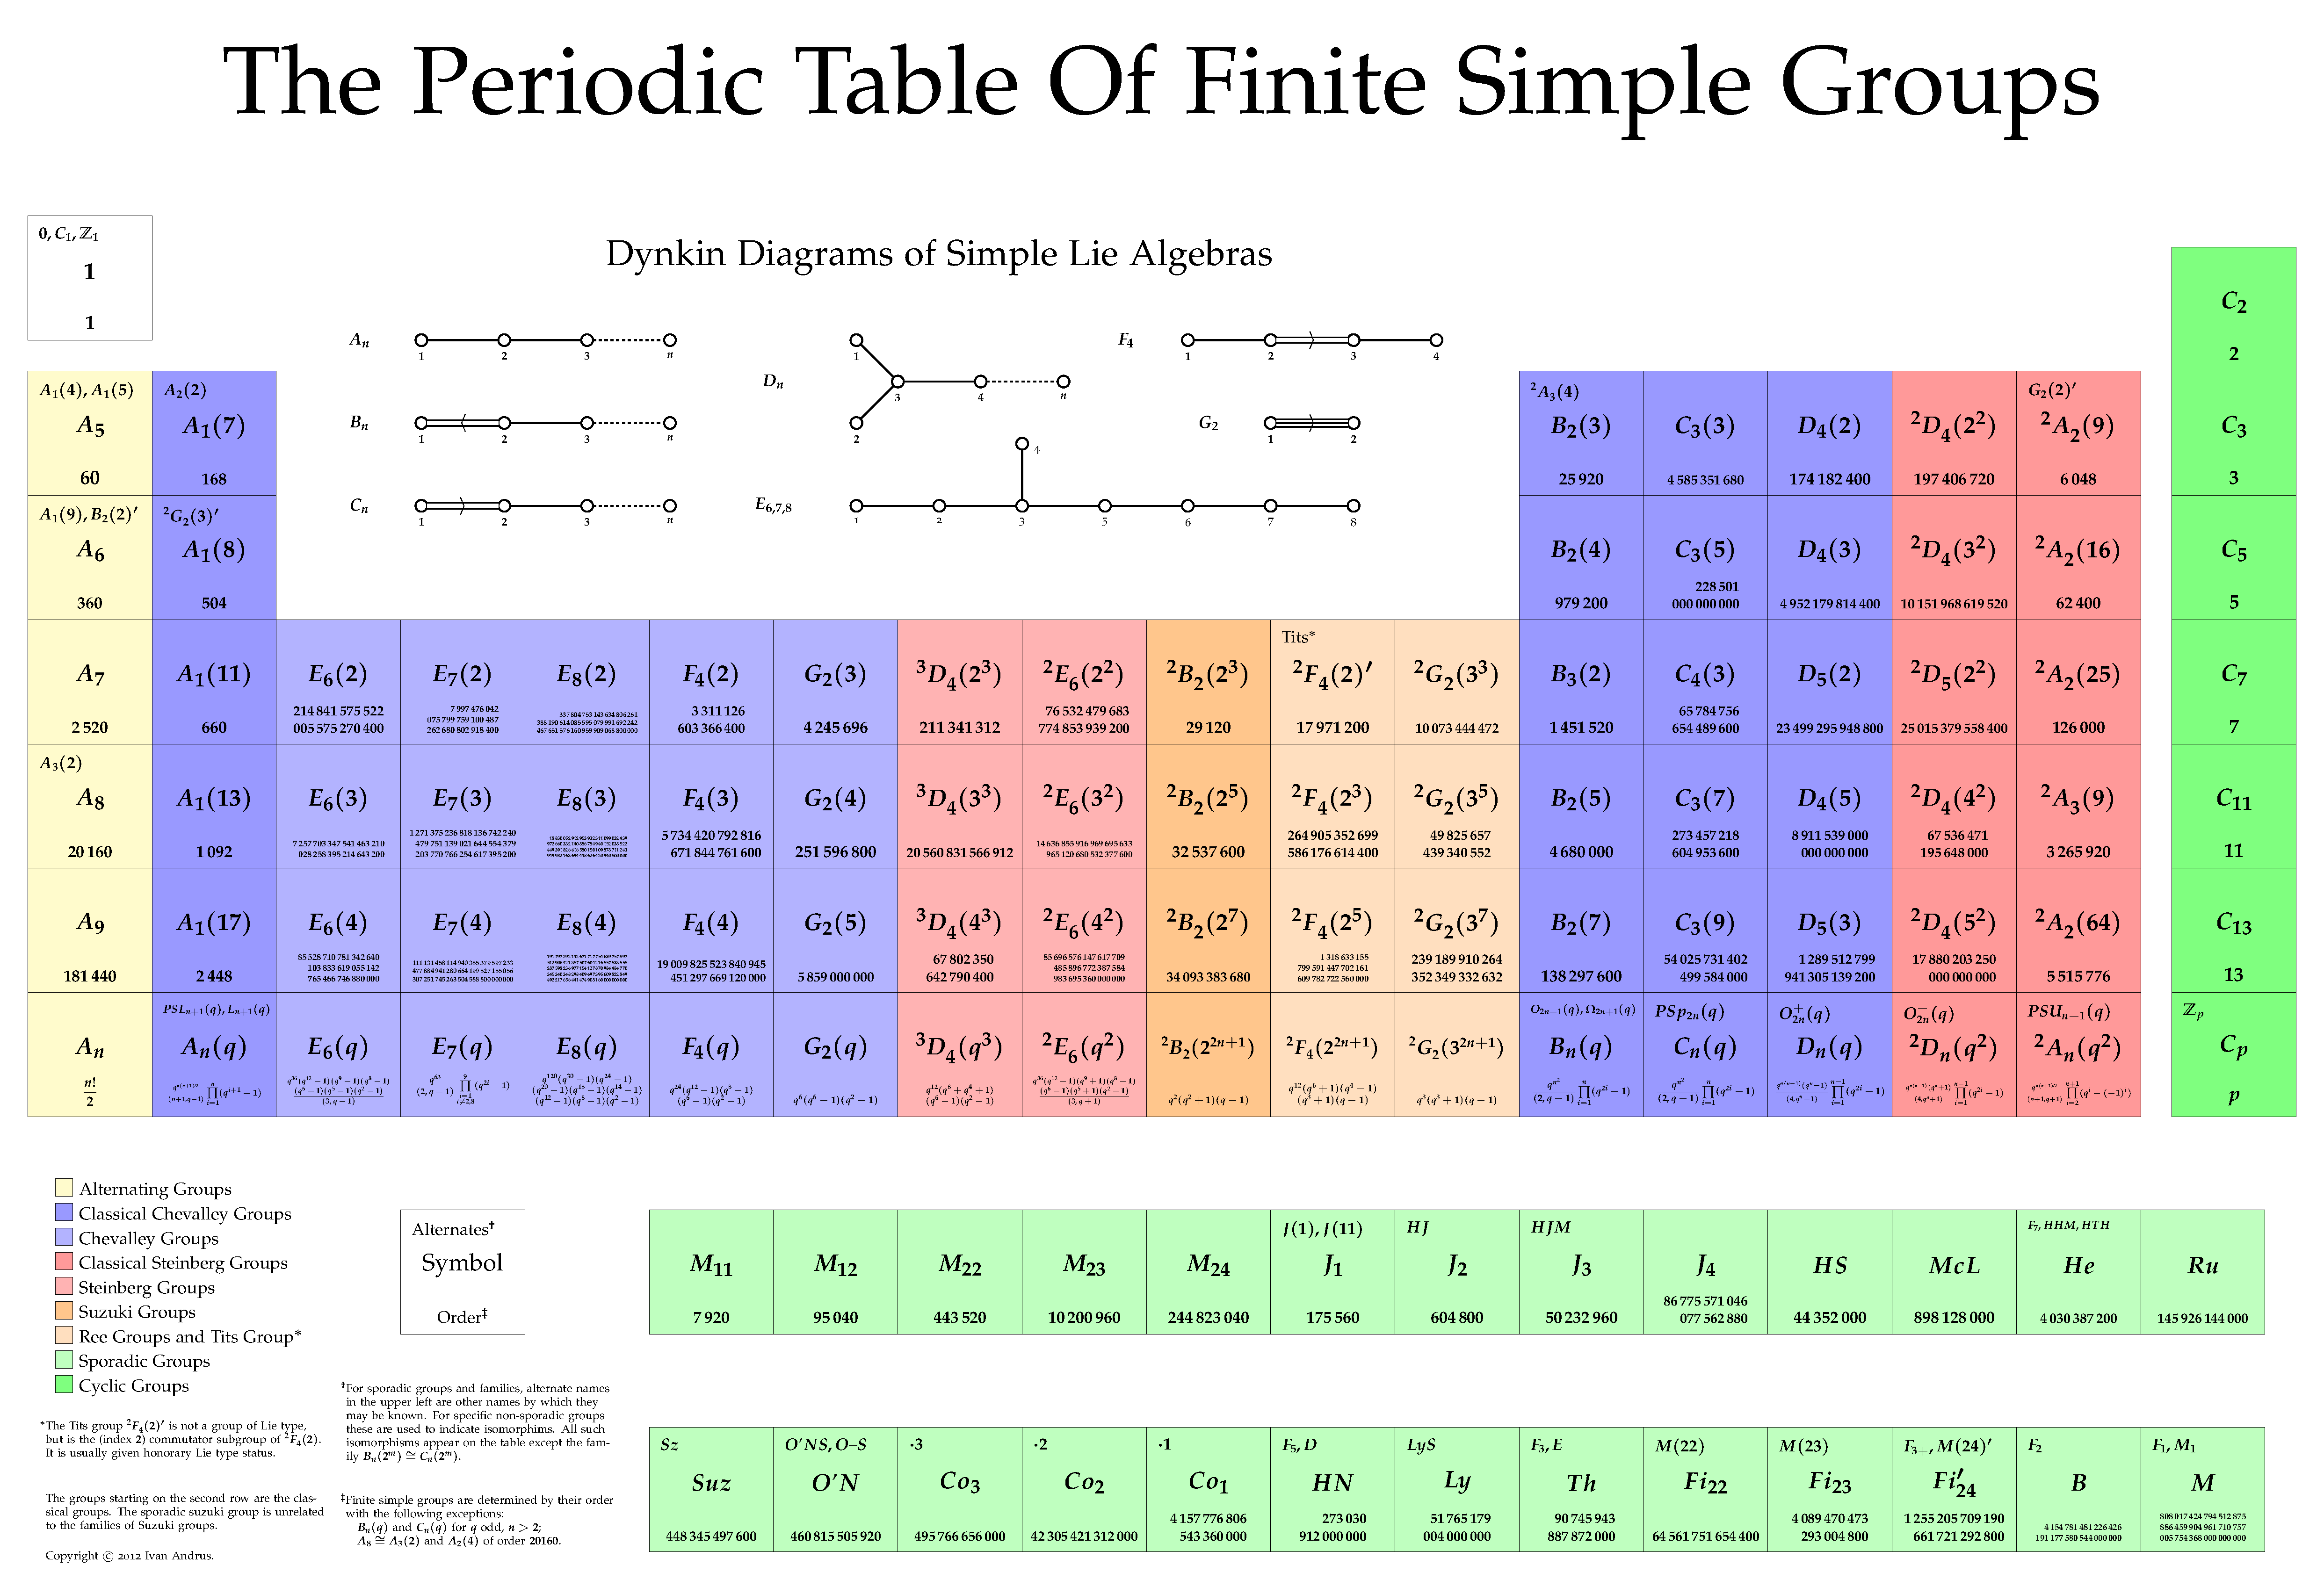
\includegraphics[scale=0.2]{Figures/CFSG}
		% 		\label{fig:CFSG}
		% 		\caption{The 18 families and 26 exceptional cases of finite simple groups.}
		% 	\end{figure}
		% \end{center}
		
		We aim to study groups via their actions on other objects. One of the most powerful ways to do this turns out to be by studying their actions on vector spaces, especially over $\mathbb C$. We assume the reader is familiar with the notion of a vector space.
		
		For any two given vector spaces, $V$ and $W$, the set of all linear transformations $T: V \to W$ is denoted by $\mathrm{Hom}(V, W)$. The set of all linear transformations $T: V \to V$ is denoted by $\mathrm{End}(V)$ (also known as endomorphisms of the vector space). Among these transformations, the invertible ones are denoted by $\mathrm{GL}(V)$, otherwise known as the \textbf{general linear group} of the space $V$. When $V$ takes the form $\mathbf k^n$ for some field $\mathbf k$ and positive integer $n$, this is denoted $\mathrm{GL}(n, \mathbf k)$. 

		 A vector space $V$ together with a group homomorphism $\rho: G \to \mathrm{GL}(V)$ is called a \textbf{representation} of $G$. Equivalently, a representation is a vector space with an action of $G$ by linear transformations. A given representation can have a \textbf{subrepresentation}, namely a subspace $V' \subseteq V$ that is preserved by the action of $G$. Every representation has itself and the $\mathbf 0$ vector as subrepresentations. These two are called the \textbf{trivial} subrepresentations. A representation with no nontrivial subrepresentations is called an \textbf{irreducible representation}. In general, we will denote the representation by $V$ alone, even though we really mean this to represent the data $(V, \rho_V)$.
		 
		A morphism between representations $V$ and $W$ is a linear map that commutes with $G$ action: $\phi(\rho_1(g)  v) = \rho_2 (g) \phi (v)$. Such maps will be called $G$\textbf{-linear}, and the set of such maps will be denoted as $\mathrm{Hom}_G(V, W)$.
		
		 
		We have the following lemma of central importance in representation theory: 
		\begin{lemma}[Schur's Lemma]
			If $V$ and $W$ are two different irreducible representations of a group $G$ over $\mathbb C$, and $\phi$ is a linear transformation from $V \to W$, then $\phi$ is either trivial (the zero map) or invertible.
			
			Further, if $V=W$ and $\rho_V=\rho_W$, then $\phi$ is either trivial or a scalar multiple of the identity. 
		\end{lemma}
		\begin{proof}
			This follows from noting that both the kernel and image of $\phi$ are subrepresentations, so must be either $\mathbf 0$ or the whole space. 
			
			The second part follows from the fact that every linear transformation over $\mathbb C$ has at least one eigenvalue $\lambda$, then one can see that $\phi - \lambda$ is also a $G$-linear transformation with a nontrivial kernel, so must be zero by the preceding.
		\end{proof}
		% The reader should be familiar with the fact that, in general, a vector space need not have an inner product, but there is a natural choice of inner product
		%
		% \begin{defn}[Semisimplicity of $\kk G$-modules
		% 	The
		% \end{defn}
		
		
		When $G$ acts on a vector space by linear endomorphism, we can not only make sense of an element $g \in G$, but also of $c g$ for $c \in \kk$. That is, we can make sense of any \emph{linear combination of elements in $G$}. This defines the \textbf{group algebra}:
		\begin{defn}[Group Algebra]
			The group algebra $\kk[G]$ for a (not necessarily finite) group $G$ is the vector space generated $\kk$-span of $\{g\}_{g \in G}$, together with multiplication of basis vectors given by group multiplication. That is, the multiplication of basis vectors $g$ and $h$ yields the basis vector $gh$.
		\end{defn}
		
		
		
		In other words we have the following equivalence\footnote{In the language of category theory, this is not just an equivalence but an \emph{isomorphism of categories}, meaning that the two categories are essentially identical with different notations.}. For a field $\kk$:
		\begin{equation*}
			\mathrm{Rep}_G \leftrightarrow \kk[G]\mathrm{-mod}
		\end{equation*}
		
		
		The representation theory of finite groups over $\mathbb C$ is particularly elegant. By \textbf{Mashke's Theorem}
		\begin{theorem}[Mashke]
			Let $\kk$ be a field of characteristic not dividing $|G|$. Then the representation theory of $G$ over $\kk$ is semisimple.
		\end{theorem}
		
		% section representation_theory_of_groups (end)
		
		\section{The Fourier Transform and Pontryagin Duality} % (fold)
		\label{sec:the_fourier_transform_and_pontryagin_duality}
		
		In this chapter, we will be working with a locally-compact (to be defined in the next part) abelian group $G$. We make the following definition:
		\begin{defn}[Unitary Character]
			For $G$ locally-compact and abelian, a \textbf{unitary character} of $G$ is a group homomorphism $\chi: G \to U(1)$.
		\end{defn}
		From this definition, we define the following group, which plays a role as a \emph{dual} to $G$. It is called the \textbf{Pontryagin dual}.
		\begin{defn}
			The set of all unitary characters $\chi$ together with multiplication given by $\chi_1 \cdot \chi_2 \in \mathrm{Hom}(G, U(1))$.
		\end{defn}
		
		\begin{eg}
			We have the following examples:
			\begin{enumerate}
				\item Let $G = S^1$, then the space of unitary characters is precisely of the form $e^{inx}: G \to U(1)$. This makes $\widehat G = \mathbb Z$.
				\item Let $G = \mathbb Z$, then $\chi(1)$ determines the representation uniquely, and so $\widehat G = U(1)$.
				\item 			Let $G = \mathbb R$, then $e^{ikx} : \mathbb R \to U(1)$ is free to have $k$ vary over $\mathbb R$ so $\widehat G = \mathbb R$.
			\end{enumerate}
			
		\end{eg}

		Notice in all these cases that $\widehat{\widehat G} \cong G$. This is in fact true more general, and we have the following theorem:
		\begin{theorem}[Pontryagin Duality]
			$G \to \widehat{\widehat G}$ is an isomorphism of groups, given by sending $g \to  g'$ which is given by $g' (\chi) = \chi (g)$.
		\end{theorem}
		
		\begin{obs}
			The $L^2$-integrable functions on $G$ have a basis given by characters. 
		\end{obs}
		\begin{eg}
			We have the following examples:
			\begin{enumerate}
				\item $f: S^1 \to \mathbb C$ has $f(\theta) = \sum_{n} a_n e^{i n \theta}$. This is known as the \textbf{Fourier series}.
				\item $f: \mathbb Z \to \mathbb C$ has $f(n) = \int_{0}^{2\pi} F(\theta) e^{i n \theta}$. This is known as the \textbf{discrete time series}.
				\item $f: \mathbb R \to \mathbb R$ has $f(x) = \int_{-\infty}^\infty \widehat{f(k)} e^{ikx}$. This is known as the \textbf{Fourier Transform}.
			\end{enumerate}
		\end{eg}
		
		Let us now try to generalize the ideas of the Fourier transform to a more direct case. It is useful to view the Fourier transform as letting us see two different sides of the same object. Let that object be the direct product of the group $G$ and $\hat G$. 
		The reason this space is worth considering is by noting that there is a unique function on this space, which we can call the \textbf{Kernel} $K: G \times \hat G \to \mathbb C$ defined by $K(g, \chi) = \chi (g)$. In the case of  $G=\mathbb R$, this function is exactly $e^{i k x}, x \in \mathbb R, k \in \widehat{ \mathbb R} = \mathbb R$, that is viewed as a function on \emph{both} time and frequency space.
		
		This space is also endowed with two obvious projections (namely to either factor of the product).		
		\[
		\begin{tikzcd}
		  & G \times \hat G \arrow[ld,"\pi_G"] \arrow[rd,swap,"\pi_{\hat G}"]&\\
		G & & \hat G
		\end{tikzcd}
		\]
		Any function $f$ on $G$ can be ``pulled back'' to a function on $G \times \hat G$, namely by ignoring the second component $f'(g, \hat g) = f(g)$. We will denote this pulled back function by $\pi_{G}^* f = f \circ \pi_G$.
		
		Further, a suitable distribution on $G \times \hat G$ can be ``pushed forward'' to either $G$ or $\hat G$ by integrating it over $\hat G$ or $G$ respectively. We will denote these by $(\pi_G)_*$ and $(\pi_{\hat G})_*$, again respectively.
		
		Now if $\hat f$ is a distribution on $\hat G$, we get that $\pi_{\hat G}^* \hat f$ is a distribution on $G \times \hat G$. This can be pushed forward to a function on $G$ by integrating over the $\hat G$ coordiantes, but because $\pi_{\hat G}^* \hat f$ is constant on the $G$-coordinate, this function will just be a constant independent of $G$.
		
		On the other hand, if we look at:
		\begin{equation}
			f (g) := {(\pi_{G})}_* ([{\pi_{\hat G}}^* \hat f] K) = \int_{\chi \in \hat G} [(\hat f \circ \pi_{\hat G}) (g, \chi)] K(g, \chi)\, d\chi
		\end{equation}
		we obtain exactly the Fourier transform. For $G = \mathbb R$ this gives us:
		\begin{equation}
			f(x) = \int_{\mathbb R} \widehat{f(k)} e^{ikx} dk.
		\end{equation}
		
		The reason that the Fourier transform finds so much use in practice is that it serves as an eigendecomposition for the derivative operator. More broadly, on $\mathbb R^n$, the eigenfunctions are plane waves $e^{i\vec k \cdot \vec x}$, which yield eigenvalues both under $\partial_x$ and also under the translation operator more generally $\vec x \mapsto \vec x + \vec y$. Any abelian group acts on itself by translation\footnote{Keep in mind that right and left action coincide for an abelian group.}. Consequently, it acts on the functions living on it, $\mathrm{Fun}(G)$, by translation $f(x) \to f(x - y)$. Note however that the unitary characters satisfy:
		\begin{equation}
			y \cdot \chi(x) = \chi(x - y) = \chi(-y) \chi(x)
		\end{equation}
		so that the characters \emph{diagonalize} the translation operator as an eigenbasis, exactly as $e^{ikx}$ did on the real line.
		
		We have just treated Fourier analysis successfully for the category of locally-compact abelian groups. The natural next question is of course
		\begin{ques}
			How does Fourier analysis look like for more general groups? That is, what is the non-abelian analogue of the Fourier transform?
		\end{ques}
		It is this stream of thought that will take us deep into the Langlands program, and ultimately into the heart of emerging ideas in theoretical physics. Already, one can see that the naive ideas from before will not hold up as well. For one, translation operators no longer commute, and so cannot be simultaneously diagonalizable with an eigenbasis of unitary characters. As we move to explore the non-abelian setting, the Pontryagin dual group $\hat G$ will be replaced by the Langlands dual group $^L G$, and of course Pontryagin duality will become a very special case of Langlands duality.
		
		It will turn out that to understand the Fourier transform in the non-abelian case, we will have to appeal to \emph{categorification}, one of the deepest aspects of twenty-first century mathematics.
		
		
		
	% section the_fourier_transform_and_pontryagin_duality (end)
	
	\section{Elementary Topology} % (fold)
	\label{sec:elementary_topology}
	
	Before we can begin a more in-depth study of symmetry and the spaces on which it acts, it is worth understanding how to study spaces in a general setting. Firstly:
	\begin{ques}
		What do we mean when we use the word ``space''?
	\end{ques}
	In this thesis alone, this word will have many meanings. The first definition we give is the starting point of topology.
	\begin{defn}[Topological Space]
		A set $X$ together with a family $\mathcal F$ of subsets of $X$ known as the \textbf{open sets} forms a \textbf{topological space} if the following conditions hold
		\begin{enumerate}
			\item The empty set $\emptyset$ and $X$ both belong to $\mathcal F$,
			\item Any union of open sets is open\footnote{It is important to understand that this can include \emph{infinite unions}},
			\item Any \emph{finite} intersection of open sets is open.
			
		\end{enumerate}
	\end{defn}
	The complement of an open set is what defines a \textbf{closed set}. It is not difficult to show that the dual properties of the above hold for closed sets, namely
	\begin{enumerate}
		\item The empty set $\emptyset$ and $X$ are both closed
		\item Any intersection of closed sets is closed
		\item Any \emph{finite} union of closed sets is closed.
	\end{enumerate}
	\begin{eg}
		The first example that we are given in high school is the real number line. The open sets are exactly the unions of the open intervals of the form $(a, b)$ while the closed sets are exactly the intersections of closed intervals of the form $[a, b]$. Note that an open set has no maximum or minimum point (i.e. the open interval $(0, 1)$ has no greatest number).
	\end{eg}
	\begin{eg}
		The previous example generalizes to $n$-dimensional space $\mathbb R^n$. Here, the open sets are generated by unions of \emph{open balls} of the form $B_a(x) := \{ \vec y : |\vec x - \vec y| < a \}$.
		
		In both of the cases, these topologies arose from the fact that these spaces are equipped with a \textbf{metric} $d(\vec x, \vec y) = |\vec x-\vec y|$ giving a notion of distance. When a metric is given, a topology can always be defined by defining open balls as above, and defining the open sets of the topology as precisely unions of open balls.
	\end{eg}
	\begin{eg}
		If all the points of a given space $X$ are open, then any subset of $X$ is also open, by virtue of being a union of points. This gives a \textbf{trivial topology} on $X$. The other trivial topology is that which consists of only $X$ and $\emptyset$ as open sets.
	\end{eg}
	
	The open sets of a space allow us to define \textbf{neighborhoods} of points. This is what allows topology to give us structure somewhat resembling the familiar structure of our (local) spacetime
	\begin{defn}[Neighborhood]
		A neighborhood of a point $p$ is a set $V$ that contains an open set $U$ containing $p$.
	\end{defn}
	This definition does not require $V$ to be open or closed. An \textbf{open neighborhood} of $p$ is any open set $U$ containing $p$. In general, open sets are supposed to play the roles of ``neighborhoods'' while closed sets are supposed to generalize the role of ``points''.
	
	Using the notions of open sets, we can define what it means for a function between two topological spaces to be \textbf{continuous}.
	\begin{defn}[Continuity of Functions between Topological Spaces]
		A function $f: X \to Y$ between the topological spaces $X$ and $Y$ is called continuous if the preimage of every open set in $V \in Y$ has $f^{-1}(V)$ open in $X$.
	\end{defn}
	It is up to the reader to check that this recovers Cauchy's epsilon-delta definition of continuity in the special case of using the Euclidean topology. The idea in topology is to identify two spaces $X$ and $Y$ as \textbf{topologically equivalent} if there are continuous functions from one to the other. We make the following definition:
	\begin{defn}[Homeomorphism]
		
	\end{defn}
	
	
	
	One of the most important properties of topological spaces is known as \textbf{compactness}. In early undergraduate classes, one may have been taught to think of compactness as being ``closed and bounded''. Indeed, this is the right way to think about it, but because ``bounded'' requires that there is a notion of distance on the space, and doesn't make much sense outside of euclidean spaces, we define compactness more generally as 
	\begin{defn}[Compact]
		A set $X$ in a topological is called compact if every open cover of $X$ contains a finite sub-cover.
	\end{defn}
	It is up to the reader (by appealing to Bolzano-Weierstrass) to confirm that this more difficult definition agrees with the naive one. 
	
	Compact spaces are especially easy to work with when performing integration, as any covering of the space into open neighborhoods can be turned into a finite number of integrations over the (usually finite-volume) neighborhoods themselves, so that one need not worry about integrals diverging. 
	
	Similarly we define
	\begin{defn}[Locally Compact]
		A space $X$ is \textbf{locally compact} if every point $x \in X$ has a compact neighborhood.
	\end{defn}
	
	Most spaces we are familiar with are locally compact. An example of a non-locally compact space is the set of rational numbers under the topology of the reals. Since all nontrivial open sets here all contain infinitely many rationals, each neighborhood must as well, and we can always construct a sequence of rationals that does not converge to a rational in the neighborhood that we are given. 
	
	
	% section elementary_topology (end)
	
	\section{Differential Geometry} % (fold)
	\label{sec:differential_geometry}
	
	The role of differential geometry in modern physics is similar to the role of the beating heart in a human body. It has become an essential ingredient in formulating physical law. Here, we will give an exposition to the ideas of differential geometry in a mathematical setting, with some motivation from physics to guide us along.
	
	\begin{defn}[Manifold]
		A manifold $M$ is a topological\footnote{More technically a topological space that is Hausdorff and second countable.} space together with the condition that every point $p$ of $M$ has an open neighborhood homeomorphic to the open unit ball $\mathbf B_n \in \rr^n$ for some $n$.
	\end{defn}
	In general, this $n$ is a local invariant, and thus constant on every connected component of $M$. For a given connected component, we will say that this component of $M$ is of dimension $n$, and that $M$ is of dimension $n$ if it has all of its components in dimension $n$. Typically, the manifolds we study will have only one connected component.
	
	
	\begin{defn}[Atlas]
		An \textbf{atlas} on a manifold $M$ is a collection of pairs $\{(U_\alpha, \varphi_{\alpha})\}_{\alpha}$ such that the $U_\alpha$ provide a cover for $M$ and the $\varphi_\alpha$ provide homeomorphisms $\varphi_\alpha: U_\alpha \to \mathbf B_n \subset \rr^n$
	\end{defn}
	Atlases are local Euclidean coordinate systems for the manifold.
	Two atlases are considered equivalent if they yield the same manifold. 
	
	\begin{defn}[Differentiable, Smooth, Analytic, and Complex Manifolds]
		A manifold $M$ equipped with an equivalence class of atlases is called a \textbf{differentiable} (resp. \textbf{smooth, analytic, complex}) \textbf{manifold} if all transition maps between charts are all differentiable (resp. smooth, have absolutely convergent Taylor expansion, holomorphic)
	\end{defn}
	
	\begin{defn}[Tangent Space, Geometric Definition]
		The tangent space to a manifold $M$ at a point $p$ is the equivalence set of 
	\end{defn}
	\begin{defn}[Tangent Space, Alternative Definition]
		The tangent space to a manifold $M$ at a point $p$ is the vector space of derivations acting on functions $f$ and evaluated at $p$.
	\end{defn}
	
	
	\begin{defn}[Vector Bundle]
		
	\end{defn}
	
	\begin{defn}[Section]
		
	\end{defn}
	
	\begin{eg}[Trivial Bundle]
		
	\end{eg}
	
	\begin{eg}[Tangent Bundle]
		The first nontrivial example of a vector bundle that one comes across is the tangent bundle of a manifold $M$, denoted by $TM$.
		
		More specifically, the tangent bundle of a sphere \textbf{Todo FINISH}
	\end{eg}
	
	\begin{obs}[Parallel Transport]
		
	\end{obs}
	
	\textbf{Something about the impossibility of transporting vectors... to be attacked when we talk about Gauge theory}
	
	\begin{defn}[Lie Derivative]
		
	\end{defn}
	
	\textbf{Work out the flow along a sphere}
	
	% section differential_geometry (end)
	
	\section{Lie Theory} % (fold)
	\label{sec:lie_theory}
		
		In physics and in mathematics, both (smooth) manifolds and groups play extremely important roles. It makes sense therefore to study their intersection: smooth manifolds that are groups. This is the study of \textbf{Lie groups}.
		\begin{defn}[Lie Group]
			A Lie group is a group $G$ that is also a manifold such that the group operations of multiplication:
			$$\mu: G \times G \to G \qquad (x, y) \to xy$$
			and inversion 
			$$^{-1} : G \to G \qquad x \to x^{-1}$$
			are smooth w.r.t. the manifold topology.
		\end{defn}
		
		Lie groups are ubiquitous in physics. $U(1)$ is a Lie group, as is the group of rotations in three dimensions, $\mathrm{SO}(3)$, or the Poincare group of symmetries in Einstein's theory of special relativity, $\mathrm{SO}(3, 1) \ltimes \mathbb R^4$.
		
		In studying the flows on manifolds, we saw that the Lie derivative allows us to measure how one flow changes along another. For Lie groups, given a vector $v_g \in T_g G$, we can canonically transport it to any other point $h \in G$ by applying the (diffeomorphism) $h g^{-1}$ to $G$ and pushing the vector forward along it to $[h g^{-1}]_* v \in T_{h} G$.
		
		WLOG, take a vector $x \in T_e G$, the tangent space at the identity. This pushforward action gives us a vector field $X \in \Gamma(G, TG)$ given by $X(g) = g_* x$. Thus, every vector defines a vector field on $G$ that is \textbf{left invariant}, meaning that $g_* X_h = X_{gh}$. Indeed we see
		\begin{prop}
			There is a one-to-one correspondence between left-invariant vector fields on $G$ and the tangent space to the identity. 
		\end{prop}
		Moreover, if two vector fields $X$ and $Y$ are left-invariant, then so is their commutator bracket $[X, Y]$. This gives us a new algebraic structure on the tangent space $T_e G$\footnote{Indeed on every tangent space, but WLOG we restrict to the identity.} given by 
		\begin{equation}
			[x, y] := \frac{d}{dt} [\exp(tx), \exp(ty)] |_{t = 0}
		\end{equation}
		this is the \textbf{Lie bracket} on the tangent space of the Lie group at the identity. We call this vector space the \textbf{Lie algebra}, denoted in fraktur by $\frak g$. It corresponds to the infinitesimal symmetries of the system, and the Lie bracket measures how one symmetry changes along the flow of the other. The example of the previous section is intimately related to the Lie group $\mathrm{SO}(3, \mathbb R)$ and its associated Lie algebra $\frak{so}(3, \mathbb R)$, more familiar to high-schoolers as the ``cross-product''.
		
		We give a few examples:
		\begin{eg}
			The Lie group of invertible linear transformations on a vector space $\mathbf k^n$, $\mathrm{GL}(n, \mathbf k)$ has the lie algebra $\frak{gl}(n, \mathbf k)$ of $n \times n$ matrices valued in $\mathbf k$, with lie bracket given by matrix commutator $[A, B] = AB - BA$.
		\end{eg}
		
		\begin{eg}
			Similarly, the Lie group of orthogonal linear transformations on a given inner product space forms is labelled by $\mathrm{SO}(n, \mathbf k)$, and gives rise to the Lie algebra $\frak{so}(n, \mathbf k)$. Because the Lie group has the requirement that $A^T A = 1$, the condition on vector in the tangent space of $\mathrm{SO}(n, \mathrm k)$ is:
			\begin{equation}
				\begin{aligned}
					\mathrm d(A^T A)  = 0 &\Rightarrow A^T dA + d{A^T} A = 0 \\
									&\Rightarrow A^{T} = - A
				\end{aligned}
			\end{equation}
		\end{eg}
		
		\begin{defn}[Ideal]
			An ideal $\frak k$ in a Lie algebra $\frak g$ is a subspace $\frak k \subseteq \frak g$ such that:
			\begin{equation}
				 \forall x \in \frak g \qquad [x, \frak k] \subseteq \frak k
			\end{equation}
			This is the analogue of an ideal for a ring. Note every Lie algebra has $\mathbf 0$ and $\frak g$ as trivial ideals. A Lie algebra with only these two trivial ideals is called \textbf{simple}.
		\end{defn}
		
		\begin{defn}[Direct Sum]
			Given any two Lie algebras $\frak g$, $\frak g'$, we define their direct sum to be a direct sum of the vector spaces $\frak g \oplus \frak g'$ with commutator bracket defined as $[(x,x'), (y, y')] = ([x, y], [x', y'])$ component-wise.
		\end{defn}
		Direct sums of Lie algebras capture independent information in that the two Lie algebras do not ``communicate with one another''.
		
		\begin{eg}
			Consider again the Lie algebra $\frak{gl}(n, \mathbf k)$, with $\mathrm{char}\, \mathbf k = 0$. Consider the 1D vector space $\frak u$ of diagonal matrices $\lambda \cdot 1$. Since diagonal matrices commute with everything, $[x, \frak k] = 0 \subseteq \frak u$, $\frak u$ is an ideal of the trivial 1-dimensional Lie algebra. Now consider the subspace of traceless matrices. Note that the vector space of matrices can be decomposed as a direct sum of the space of traceless matrices and this 1D space. We suggestively denote the space of traceless matrices by $\frak{sl}(n, \mathbf k)$.
			
			It is easy to check that when $\mathrm{char}\, \mathbf k = 0$, the Lie algebra splits into a direct sum $\frak{gl}(n, \mathbf k) = \frak{sl}(n, \mathbf k) \oplus \frak u$ . Less obvious is the fact that $\frak{sl}(n, \mathbf k)$ is in fact simple in this case.
		\end{eg}
		
		Now let us try to build an analogy to the previous examples of semisimplicity, and nilpotency. The reader should take a moment to understand why these definitions are the `right' ones to consider.
		
		\begin{defn}[Semisimple Lie Algebras]
			A Lie algebra is \textbf{semisimple} if it is a direct sum of simple Lie algebras.
		\end{defn}
		
		\begin{defn}[Nilpotent Lie Algebras]
			Define $\gg_{(1)} := [\gg, \gg]$ and iteratively $\gg_{(i+1)} = [\gg, \gg_{(i)}]$.
			A Lie algebra is \textbf{nilpotent} if $\gg_{(k)} = 0$ for some $1 \leq k \leq \dim \gg$.
		\end{defn}
		
		The representation theory of semisimple Lie algebras is particularly elegant, and in many ways mirrors the representation theory of finite groups, but with a much simpler and more elegant classification structure. 
		
		To study the representation theory of Lie algebras, recall the Jordan normal form. 
		
		\begin{defn}[Cartan Subalgebra]
			A \textbf{Cartan subalgebra} of a Lie algebra $\frak g$ is a maximal abelian subalgebra.
		\end{defn}
		From a physical 
		
		\textbf{Adjoint representation stuff}
		
		\begin{prop}
			If $\frak g$ is a Lie algebra over an algebraically closed field, then any two Cartan subalgebras are conjugate by $\Ad_G$ action. In particular, all Cartan subalgebras have the same dimension, known as the \textbf{rank} of $\frak g$.
		\end{prop}
		
		\textbf{Root system stuff}
		
		
	% section lie_theory (end)
	
	\section{Algebraic Topology} % (fold)
	\label{sec:algebraic_topology}
	
	Just as we have before studied groups by their actions on spaces, it is also equally fruitful to study topological spaces $X$ by finding groups associated to them. The easiest example of this comes from the theory of the fundamental group $\pi_1 (X)$ and then again from the study of the homology and cohomology of $X$. We will outline these theories briefly here and direct the reader to \cite{hatcher} for a deeper expository text.
	
	% section algebraic_topology (end)
	


	\section{Elementary Algebraic Geometry} % (fold)
	\label{sec:elementary_algebraic_geometry}

	% section elementary_algebraic_geometry (end)
	
	\section{Intermediate Algebraic Geometry} % (fold)
	\label{sec:intermediate_algebraic_geometry}
	
	% section intermediate_algebraic_geometry (end)